% Gabarit pandoc des corrigés publiés (brut et guidé). Contenu sans marque ni nom de site.
% Compilation : lualatex (latexmk -lualatex).
% Le Markdown reste la source unique : ne pas éditer ce fichier .tex à la main.
\documentclass[11pt,a4paper]{article}

% --- Moteur, polices (Latin Modern) et langue ---------------------------------
\usepackage{iftex}
\ifLuaTeX\else\errmessage{Ce document se compile avec lualatex}\fi
\usepackage{amsmath,amssymb,mathtools}
\usepackage{fontspec}
% mathrm=sym : \mathrm prend ses glyphes dans la police mathématique (ℓ, μ, Ω), comme KaTeX.
\usepackage[math-style=TeX,bold-style=TeX,mathrm=sym]{unicode-math}
% Repli pour les glyphes absents de Latin Modern (indices et exposants Unicode,
% flèches, filets des schémas en texte, symboles) : DejaVu, puis Latin Modern Math
% (ℓ, lettres mathématiques Unicode des légendes).
\directlua{
  luaotfload.add_fallback("repliTexte", {"DejaVuSerif:mode=harf;", "DejaVuSans:mode=harf;", "file:latinmodern-math.otf:mode=harf;"})
  luaotfload.add_fallback("repliMono", {"DejaVuSansMono:mode=harf;", "DejaVuSans:mode=harf;", "file:latinmodern-math.otf:mode=harf;"})
}
\setmainfont{Latin Modern Roman}[RawFeature={fallback=repliTexte}]
\setsansfont{Latin Modern Sans}[RawFeature={fallback=repliTexte}]
\setmonofont{Latin Modern Mono}[RawFeature={fallback=repliMono}]
\setmathfont{Latin Modern Math}
\usepackage[french]{babel}
\frenchsetup{SmallCapsFigTabCaptions=false}

% --- Mise en page --------------------------------------------------------------
\usepackage[a4paper,margin=2.2cm,headheight=14pt,footskip=1.2cm]{geometry}
\usepackage{microtype}
\setlength{\emergencystretch}{4em}
\tolerance=1500
\setlength{\parindent}{0pt}
\setlength{\parskip}{0.55\baselineskip plus 2pt minus 1pt}
\usepackage{xcolor}
% Gris nommés : babel-french rend « ! » actif dans le document.
\definecolor{gris2}{gray}{0.98}
\definecolor{gris3}{gray}{0.97}
\definecolor{gris5}{gray}{0.95}
\definecolor{gris35}{gray}{0.65}
\definecolor{gris40}{gray}{0.60}
\definecolor{gris45}{gray}{0.55}
\definecolor{gris50}{gray}{0.50}
\definecolor{gris55}{gray}{0.45}
\definecolor{gris60}{gray}{0.40}
\definecolor{gris65}{gray}{0.35}
\definecolor{gris70}{gray}{0.30}
\definecolor{gris80}{gray}{0.20}
\definecolor{gris85}{gray}{0.15}
\usepackage{graphicx}
\usepackage{float}
\usepackage{caption}
\captionsetup{font=small,labelformat=empty,justification=centering}
\usepackage{booktabs,longtable,array,multirow,calc}
\usepackage{siunitx}
\sisetup{locale=FR}
\usepackage[version=4]{mhchem}
\usepackage{listings}
\usepackage{fancyhdr}
\usepackage{lastpage}
\usepackage[most]{tcolorbox}
\usepackage{enumitem}
\setlist{nosep,leftmargin=*,topsep=2pt}
\usepackage[hidelinks,unicode]{hyperref}
\usepackage{bookmark}
\hypersetup{pdftitle={CCINP PC — Mathématiques 2026},pdfauthor={Rédigé par IA},pdfcreator={LaTeX},pdfsubject={Corrigé brut}}
\usepackage{xurl}

% --- Pandoc : listes, tableaux, figures ----------------------------------------
\providecommand{\passthrough}[1]{#1}
\providecommand{\tightlist}{\setlength{\itemsep}{0pt}\setlength{\parskip}{0pt}}

\makeatletter
\def\maxwidth{\ifdim\Gin@nat@width>\linewidth\linewidth\else\Gin@nat@width\fi}
\def\maxheight{\ifdim\Gin@nat@height>0.55\textheight 0.55\textheight\else\Gin@nat@height\fi}
\makeatother
\setkeys{Gin}{width=\maxwidth,height=\maxheight,keepaspectratio}
\setcounter{secnumdepth}{-\maxdimen}
\providecommand{\pandocbounded}[1]{#1}

% --- Code (listings) -----------------------------------------------------------
\lstset{
  basicstyle=\ttfamily\small,
  columns=fullflexible,
  keepspaces=true,
  breaklines=true,
  breakatwhitespace=false,
  postbreak=\mbox{\textcolor{gris50}{$\hookrightarrow$}\space},
  frame=single,
  rulecolor=\color{gris35},
  framesep=4pt,
  xleftmargin=5pt,xrightmargin=5pt,
  backgroundcolor=\color{gris3},
  keywordstyle=\bfseries,
  commentstyle=\color{gris65},
  stringstyle=\color{gris80},
  showstringspaces=false,
  tabsize=4,
  extendedchars=true,
  aboveskip=6pt,belowskip=6pt,
}

% --- Macros des corrigés (KaTeX ↔ LaTeX) ---------------------------------------
% Les corrigés sont écrits pour KaTeX : on définit ici ce que KaTeX connaît et
% que LaTeX n'a pas, sans jamais retoucher le Markdown.
\providecommand{\R}{\mathbb{R}}
\providecommand{\N}{\mathbb{N}}
\providecommand{\Z}{\mathbb{Z}}
\providecommand{\Q}{\mathbb{Q}}
\providecommand{\C}{\mathbb{C}}
\providecommand{\dd}{\mathrm{d}}
\providecommand{\llbracket}{\lBrack}
\providecommand{\rrbracket}{\rBrack}
\providecommand{\lBrace}{\lbrace}
\providecommand{\rBrace}{\rbrace}
\providecommand{\Box}{\square}
\providecommand{\Diamond}{\lozenge}
\providecommand{\varnothing}{\emptyset}
\providecommand{\argmax}{\operatorname*{arg\,max}}
\providecommand{\argmin}{\operatorname*{arg\,min}}
\renewcommand{\leq}{\leqslant}
\renewcommand{\geq}{\geqslant}

% Équation hors texte : réduite à la largeur de la ligne si elle déborde.
\newsavebox{\boiteequation}
\newcommand{\equationajustee}[1]{%
  \sbox{\boiteequation}{$\displaystyle #1$}%
  \ifdim\wd\boiteequation>\linewidth
    \[\resizebox{\linewidth}{!}{\usebox{\boiteequation}}\]%
  \else
    \[#1\]%
  \fi}

% --- Encadrés pédagogiques (sobres, lisibles en noir et blanc) -----------------
\tcbset{
  encadre/.style={
    enhanced,breakable,sharp corners,
    colback=white,colframe=gris55,
    boxrule=0.4pt,leftrule=2.2pt,
    left=6pt,right=6pt,top=3pt,bottom=3pt,
    before skip=6pt,after skip=6pt,
    fonttitle=\bfseries\small,coltitle=black,
    attach title to upper,after title={\quad},
    parbox=false,
  }
}
\newtcolorbox{indication}[1]{encadre,colframe=gris45,colback=gris2,title={Indication~#1}}
\newtcolorbox{methode}{encadre,colframe=gris70,title={Méthode}}
\newtcolorbox{piege}{encadre,colframe=gris85,boxrule=0.8pt,leftrule=2.2pt,title={Piège}}
\newtcolorbox{jury}{encadre,colframe=gris60,colback=gris5,title={Jury}}
\newtcolorbox{encadrenote}{encadre,colframe=gris40}

% --- Titres de section ---------------------------------------------------------
\usepackage{titlesec}
\titleformat{\section}{\Large\bfseries}{}{0pt}{}
\titleformat{\subsection}{\large\bfseries}{}{0pt}{}
\titleformat{\subsubsection}{\normalsize\bfseries}{}{0pt}{}
\titlespacing*{\section}{0pt}{14pt plus 4pt minus 2pt}{6pt}
\titlespacing*{\subsection}{0pt}{10pt plus 3pt minus 2pt}{4pt}
\titlespacing*{\subsubsection}{0pt}{8pt plus 2pt minus 2pt}{2pt}

% --- En-tête et pied de page ---------------------------------------------------
\pagestyle{fancy}
\fancyhf{}
\fancyhead[L]{\small\textsc{Corrigé brut} · CCINP PC}
\fancyhead[R]{\small Maths 2026}
\fancyfoot[L]{\footnotesize Corrigé rédigé par IA, non officiel}
\fancyfoot[R]{\footnotesize \thepage\,/\,\pageref*{LastPage}}
\renewcommand{\headrulewidth}{0.4pt}
\renewcommand{\footrulewidth}{0pt}
\fancypagestyle{plain}{\fancyhf{}\fancyfoot[R]{\footnotesize \thepage\,/\,\pageref*{LastPage}}\fancyfoot[L]{\footnotesize Corrigé rédigé par IA, non officiel}\renewcommand{\headrulewidth}{0pt}}

\begin{document}
\thispagestyle{plain}
\begin{center}
  {\small\scshape Corrigé brut}\par\smallskip
  {\LARGE\bfseries CCINP PC — Mathématiques 2026\par}\medskip
  {\large CCINP · PC · Maths · 2026\par}
\end{center}
\vspace{2pt}\hrule\vspace{8pt}

\emph{Corrigé rédigé par IA, non officiel. Signalez toute erreur.}

Épreuve PC1M, durée 4 heures, calculatrices interdites. Trois exercices indépendants, 37 questions.

Convention : pour \(B\in\mathcal M_p(\mathbb R)\), on pose \(\chi_B(X)=\det(XI_p-B)\). C'est la convention compatible avec la formule de la Q6. \(\mathrm{Sp}(B)\) désigne l'ensemble des valeurs propres de \(B\).

\begin{center}\rule{0.5\linewidth}{0.5pt}\end{center}

Exercice 1 --- Réduction de matrices par blocs

\hypertarget{partie-i---uxe9tude-dune-premiuxe8re-forme}{%
\section{Partie I - Étude d'une première forme}\label{partie-i---uxe9tude-dune-premiuxe8re-forme}}

Ici \(M=\begin{pmatrix}A&A\\A&A\end{pmatrix}\).

\hypertarget{i.1---uxe9tude-dun-exemple}{%
\subsection{I.1 - Étude d'un exemple}\label{i.1---uxe9tude-dun-exemple}}

\(n=2\), \(A=\mathrm{diag}(1,2)\), donc
\equationajustee{M=\begin{pmatrix}1&0&1&0\\0&2&0&2\\1&0&1&0\\0&2&0&2\end{pmatrix}.}

\textbf{Q1.} \(A\) est diagonale, donc symétrique. Par blocs,
\equationajustee{M^\top=\begin{pmatrix}A^\top&A^\top\\A^\top&A^\top\end{pmatrix}=M.}
La matrice \(M\) est symétrique réelle ; d'après le théorème spectral, elle est diagonalisable (dans une base orthonormée).
\equationajustee{\boxed{M\text{ est diagonalisable.}}}

\textbf{Q2.} Pour \(x,y\in\mathbb R^2\), on a par blocs
\equationajustee{M\begin{pmatrix}x\\y\end{pmatrix}=\begin{pmatrix}A(x+y)\\A(x+y)\end{pmatrix}.}

\begin{itemize}
\tightlist
\item
  Pour \(y=-x\), on obtient \(0\). Le sous-espace \(G=\{(x,-x)\,;\,x\in\mathbb R^2\}\), de dimension \(2\), est donc inclus dans \(\ker M\).
  Les colonnes 1 et 3 de \(M\) sont égales, de même que les colonnes 2 et 4, et les colonnes 1 et 2 sont libres. Donc \(\mathrm{rg}\,M=2\).
  Par le théorème du rang, \(\dim\ker M=2\), d'où \(\ker M=G\).
\item
  Pour \(y=x\), on obtient \(M(x,x)=(2Ax,2Ax)\). Posons \(u_1=(1,0,1,0)\) et \(u_2=(0,1,0,1)\). Alors \(Mu_1=2u_1\) et \(Mu_2=4u_2\).
\end{itemize}

La somme des dimensions des sous-espaces propres trouvés vaut \(2+1+1=4\) : ce sont tous les sous-espaces propres.
\equationajustee{\boxed{\mathrm{Sp}(M)=\{0,2,4\}}}
avec \(\dim E_0(M)=2\) et \(\dim E_2(M)=\dim E_4(M)=1\). C'est cohérent avec la Q6 :
\equationajustee{\begin{aligned}
\chi_M(\lambda)&=\lambda^2\cdot4\left(\tfrac\lambda2-1\right)\left(\tfrac\lambda2-2\right)\\
&=\lambda^2(\lambda-2)(\lambda-4).
\end{aligned}}

\textbf{Q3.} \(M\) est symétrique (Q1). Soit \(X=\begin{pmatrix}x\\y\end{pmatrix}\in\mathbb R^4\). Posons \(z=x+y=(z_1,z_2)\) et utilisons \(A^\top=A\) :
\equationajustee{\begin{aligned}
X^\top MX&=x^\top A(x+y)+y^\top A(x+y)\\
&=z^\top Az\\
&=z_1^2+2z_2^2\\
&\ge0 .
\end{aligned}}
Donc \(M\in\mathcal S_4^+(\mathbb R)\). Elle n'est pas définie positive : pour \(X_0=(1,0,-1,0)\neq0\), on a \(z=0\), donc \(X_0^\top MX_0=0\). De façon équivalente, \(0\in\mathrm{Sp}(M)\).
\equationajustee{\boxed{M\text{ est \text{symétrique} positive, mais pas \text{définie} positive.}}}

\hypertarget{i.2---ruxe9duction-de-la-matrice-m}{%
\subsection{\texorpdfstring{I.2 - Réduction de la matrice \(M\)}{I.2 - Réduction de la matrice M}}\label{i.2---ruxe9duction-de-la-matrice-m}}

\textbf{Q4.} Posons \(Q=\frac12\begin{pmatrix}I_n&-I_n\\I_n&I_n\end{pmatrix}\). Le produit par blocs (les blocs sont des matrices de \(\mathcal M_n(\mathbb R)\), multipliées comme telles) donne
\equationajustee{\begin{aligned}
PQ&=\frac12\begin{pmatrix}I_n+I_n&-I_n+I_n\\-I_n+I_n&I_n+I_n\end{pmatrix}\\
&=I_{2n}.
\end{aligned}}
En dimension finie, une matrice carrée qui admet un inverse à droite est inversible, d'inverse celui-ci. Donc \(P\) est inversible et
\equationajustee{\boxed{P^{-1}=\frac12\begin{pmatrix}I_n&-I_n\\I_n&I_n\end{pmatrix}.}}
(Le calcul de \(QP\) donne aussi \(I_{2n}\).)

\textbf{Q5.} On calcule par blocs :
\equationajustee{\begin{aligned}
MP&=\begin{pmatrix}A&A\\A&A\end{pmatrix}\begin{pmatrix}I_n&I_n\\-I_n&I_n\end{pmatrix}\\
&=\begin{pmatrix}O_n&2A\\O_n&2A\end{pmatrix},
\end{aligned}}
puis
\equationajustee{\begin{aligned}
P^{-1}MP&=\frac12\begin{pmatrix}I_n&-I_n\\I_n&I_n\end{pmatrix}\begin{pmatrix}O_n&2A\\O_n&2A\end{pmatrix}\\
&=\frac12\begin{pmatrix}O_n&O_n\\O_n&4A\end{pmatrix}\\
&=D.
\end{aligned}}
\equationajustee{\boxed{P^{-1}MP=D=\begin{pmatrix}O_n&O_n\\O_n&2A\end{pmatrix},\ \text{donc } M \text{ est semblable \text{à} } D.}}

\begin{figure}[H]
\centering
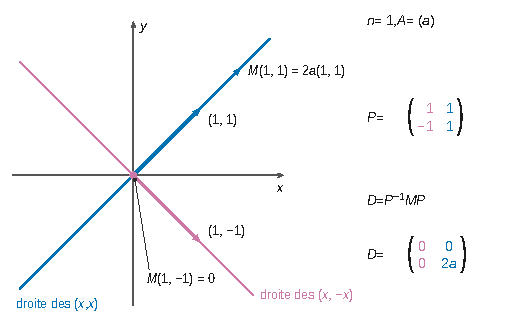
\includegraphics{figures/q05-action-de-m-cas-n1.pdf}
\caption*{Figure 1 --- Cas modèle n = 1, A = (a) : les colonnes de P dirigent la
droite des (x, −x), envoyée sur 0, et celle des (x, x), dilatée d'un
facteur 2a ; d'où P⁻¹MP = D}
\end{figure}

\textbf{Q6.} Deux matrices semblables ont le même polynôme caractéristique, donc \(\chi_M=\chi_D\) (Q5). Soit \(\lambda\in\mathbb R\) :
\equationajustee{\lambda I_{2n}-D=\begin{pmatrix}\lambda I_n&O_n\\O_n&\lambda I_n-2A\end{pmatrix}.}
La première colonne a pour seul coefficient éventuellement non nul \(\lambda\), en position \((1,1)\). En développant \(n\) fois de suite selon la première colonne, puis par homogénéité du déterminant sur \(\mathcal M_n(\mathbb R)\) :
\equationajustee{\begin{aligned}
\det(\lambda I_{2n}-D)&=\lambda^n\det(\lambda I_n-2A)\\
&=\lambda^n\,2^n\det\!\left(\tfrac\lambda2I_n-A\right).
\end{aligned}}
D'où, pour tout \(\lambda\in\mathbb R\),
\equationajustee{\boxed{\chi_M(\lambda)=\lambda^n\,2^n\,\chi_A\!\left(\frac\lambda2\right).}}
Puisque \(2^n\ne0\), on a \(\chi_M(\lambda)=0\) si et seulement si \(\lambda=0\) ou \(\lambda/2\in\mathrm{Sp}(A)\).

Comme \(n\ge1\), le réel \(0\) est toujours valeur propre de \(M\). Les autres valeurs propres sont les \textbf{doubles} de celles de \(A\) :
\equationajustee{\boxed{\mathrm{Sp}(M)=\{0\}\cup\{2\mu\,;\,\mu\in\mathrm{Sp}(A)\}.}}

\textbf{Q7.} Par récurrence immédiate, pour \(k\ge1\),
\equationajustee{D^k=\begin{pmatrix}O_n&O_n\\O_n&(2A)^k\end{pmatrix},}
et \(D^0=I_{2n}\). Pour \(R=\sum_k r_kX^k\in\mathbb R[X]\), on en déduit
\equationajustee{R(D)=\begin{pmatrix}R(0)I_n&O_n\\O_n&R(2A)\end{pmatrix}.}
Prenons \(R=Q\!\left(\frac X2\right)=\sum_{k=0}^dq_k2^{-k}X^k\). Alors \(R(0)=Q(0)\), et
\equationajustee{\begin{aligned}
R(2A)&=\sum_{k=0}^dq_k2^{-k}2^kA^k\\
&=Q(A).
\end{aligned}}
Donc
\equationajustee{Q\!\left(\tfrac X2\right)(D)=\begin{pmatrix}Q(0)I_n&O_n\\O_n&Q(A)\end{pmatrix}.}
Cette matrice est nulle si et seulement si ses deux blocs diagonaux le sont. Puisque \(n\ge1\), cela équivaut à \(Q(0)=0\) et \(Q(A)=O_n\).
\equationajustee{\boxed{\text{(i)}\iff\text{(ii)}.}}

\textbf{Q8.} \(M\) et \(D\) sont semblables (Q5), donc \(M\) est diagonalisable si et seulement si \(D\) l'est. On utilise la caractérisation : une matrice est diagonalisable si et seulement si elle admet un polynôme annulateur scindé à racines simples.

\emph{Si \(A\) est diagonalisable.} Soit \(\pi\) un polynôme annulateur de \(A\) scindé à racines simples, par exemple \(\pi=\prod_{\mu\in\mathrm{Sp}(A)}(X-\mu)\).

On pose \(Q=\pi\) si \(\pi(0)=0\), et \(Q=X\pi\) sinon.

Le polynôme \(Q\) est scindé à racines simples : dans le second cas, la racine \(0\) ajoutée n'était pas racine de \(\pi\).

De plus, \(Q(A)=O_n\) et \(Q(0)=0\). Par la Q7, \(Q(X/2)\) annule \(D\).

Si \(Q=c\prod_i(X-\alpha_i)\) avec des \(\alpha_i\) distincts, alors
\equationajustee{Q\!\left(\tfrac X2\right)=c\,2^{-\deg Q}\prod_i(X-2\alpha_i),}
qui est scindé à racines simples. Donc \(D\) est diagonalisable.

\emph{Si \(D\) est diagonalisable.} Soit \(R\) un polynôme annulateur de \(D\) scindé à racines simples : \(R=c\prod_j(X-\nu_j)\), avec des \(\nu_j\) distincts. On pose
\equationajustee{Q=R(2X)=c\,2^{\deg R}\prod_j\left(X-\tfrac{\nu_j}2\right).}
Il est scindé à racines simples, et \(Q(X/2)=R\) annule \(D\). Par la Q7, \(Q(A)=O_n\). Donc \(A\) est diagonalisable.
\equationajustee{\boxed{M\text{ est diagonalisable}\iff A\text{ est diagonalisable.}}}

\hypertarget{partie-ii---uxe9tude-dune-seconde-forme}{%
\section{Partie II - Étude d'une seconde forme}\label{partie-ii---uxe9tude-dune-seconde-forme}}

Ici \(M=\begin{pmatrix}A&A\\O_n&A\end{pmatrix}\).

\textbf{Q9.} Récurrence sur \(k\).

\begin{itemize}
\tightlist
\item
  Initialisation, \(k=0\) : \(M^0=I_{2n}=\begin{pmatrix}I_n&0\cdot I_n\\O_n&I_n\end{pmatrix}\), et \(A^0=I_n\).
\item
  Hérédité : si \(M^k=\begin{pmatrix}A^k&kA^k\\O_n&A^k\end{pmatrix}\), alors
\end{itemize}

\equationajustee{\begin{aligned}
M^{k+1}&=M^kM\\
&=\begin{pmatrix}A^k&kA^k\\O_n&A^k\end{pmatrix}\begin{pmatrix}A&A\\O_n&A\end{pmatrix}\\
&=\begin{pmatrix}A^{k+1}&A^{k+1}+kA^{k+1}\\O_n&A^{k+1}\end{pmatrix}\\
&=\begin{pmatrix}A^{k+1}&(k+1)A^{k+1}\\O_n&A^{k+1}\end{pmatrix}.
\end{aligned}}
\equationajustee{\boxed{\forall k\in\mathbb N,\quad M^k=\begin{pmatrix}A^k&kA^k\\O_n&A^k\end{pmatrix}.}}

\textbf{Q10.} Soit \(Q=\sum_{k=0}^dq_kX^k\). Par linéarité et d'après la Q9 :
\equationajustee{Q(M)=\sum_{k=0}^dq_kM^k=\begin{pmatrix}\sum_kq_kA^k&\sum_{k\ge1}kq_kA^k\\O_n&\sum_kq_kA^k\end{pmatrix}.}
Or
\equationajustee{\begin{aligned}
AQ'(A)&=A\sum_{k\ge1}kq_kA^{k-1}\\
&=\sum_{k\ge1}kq_kA^k,
\end{aligned}}
d'où
\equationajustee{\boxed{Q(M)=\begin{pmatrix}Q(A)&AQ'(A)\\O_n&Q(A)\end{pmatrix}.}}

\textbf{Q11.} On a \(S(M)=O_{2n}\). Par la Q10, bloc par bloc :
\equationajustee{\begin{cases}S(A)=O_n,\\ AS'(A)=O_n.\end{cases}\qquad(\dagger)}
\(S\) est un polynôme annulateur de \(A\) scindé à racines simples : par le cours, \(A\) est diagonalisable.

Écrivons \(A=P\Delta P^{-1}\) avec \(\Delta=\mathrm{diag}(\mu_1,\dots,\mu_n)\), où les \(\mu_i\) sont les valeurs propres de \(A\) répétées.

Alors \(A^k=P\Delta^kP^{-1}\) pour tout \(k\), et par linéarité
\equationajustee{S'(A)=P\,\mathrm{diag}\big(S'(\mu_1),\dots,S'(\mu_n)\big)\,P^{-1}.}
\equationajustee{\boxed{S'(A)\text{ est diagonalisable et }\mathrm{Sp}(S'(A))=\{S'(\mu)\,;\,\mu\in\mathrm{Sp}(A)\}.}}

\textbf{Q12.} Soit \(\mu\in\mathrm{Sp}(A)\) et \(x\ne0\) un vecteur propre associé. De \(0=S(A)x=S(\mu)x\), on tire \(S(\mu)=0\) : les valeurs propres de \(A\) sont des racines de \(S\).

Écrivons \(S=c\prod_{i=1}^r(X-\alpha_i)\), avec \(c\neq0\) et des \(\alpha_i\) distincts. Alors
\equationajustee{S'(\alpha_j)=c\prod_{i\ne j}(\alpha_j-\alpha_i)\ne0 .}
Ainsi \(S'\) ne s'annule en aucune racine de \(S\), donc \(S'(\mu)\ne0\) pour tout \(\mu\in\mathrm{Sp}(A)\). Par la Q11, \(0\notin\mathrm{Sp}(S'(A))\).
\equationajustee{\boxed{S'(A)\text{ est inversible.}}}
En multipliant la seconde relation de \((\dagger)\) à droite par \(S'(A)^{-1}\), on obtient \(A=O_n\). Réciproquement, si \(A=O_n\), alors \(M=O_{2n}\) est diagonale.
\equationajustee{\boxed{M\text{ est diagonalisable}\iff A=O_n.}}

\begin{center}\rule{0.5\linewidth}{0.5pt}\end{center}

Exercice 2 --- Autour de la loi géométrique

\(X_k\hookrightarrow\mathcal G(p)\) : \(X_k(\Omega)=\mathbb N^*\) et \(P(X_k=j)=pq^{j-1}\).

\hypertarget{partie-i---uxe9tude-de-la-variable-aluxe9atoire-s_n}{%
\section{\texorpdfstring{Partie I - Étude de la variable aléatoire \(S_n\)}{Partie I - Étude de la variable aléatoire S\_n}}\label{partie-i---uxe9tude-de-la-variable-aluxe9atoire-s_n}}

\textbf{Q13.} Les \(X_k\) sont à valeurs dans \(\mathbb N^*\), donc \(S_n\) est à valeurs entières et \(S_n\ge n\). Réciproquement, soit \(k\ge n\). Par indépendance,
\equationajustee{\begin{aligned}
P(S_n=k)&\ge P\big((X_1=k-n+1)\cap(X_2=1)\cap\dots\cap(X_n=1)\big)\\
&=pq^{k-n}\,p^{n-1}\\
&>0.
\end{aligned}}
\equationajustee{\boxed{S_n(\Omega)=[\![n,+\infty[\![ .}}

\textbf{Q14.} On a \(E(X_1)=\frac1p\) et \(V(X_1)=\frac q{p^2}\). L'espérance est linéaire. Les \(X_k\) sont indépendantes, donc la variance de leur somme est la somme des variances :
\equationajustee{\boxed{\begin{aligned}E(S_n)&=\frac np,\\ V(S_n)&=\frac{nq}{p^2}.\end{aligned}}}

\textbf{Q15.} Par définition, le rayon de convergence \(R\) est la borne supérieure des \(r\ge0\) tels que la suite \((P(Y=k)\,r^k)_k\) soit bornée.

Pour \(r=1\), on a \(0\le P(Y=k)\le1\) pour tout \(k\) : la suite \((P(Y=k)\,1^k)\) est bornée. Donc \(\boxed{R\ge1}\).

(On peut aussi dire que la série converge en \(t=1\), de somme \(1\), ce qui donne \(R\ge1\) par le lemme d'Abel.)

\textbf{Q16.} Les \(X_k\) sont mutuellement indépendantes. Par le lemme des coalitions, \(S_{m-1}\) et \(X_m\) sont indépendantes pour \(2\le m\le n\).

Soient \(U,V\) deux variables indépendantes à valeurs dans \(\mathbb N\), et \(t\in\,]-1,1[\). Les variables \(t^U\) et \(t^V\) sont indépendantes et bornées, donc \(G_{U+V}(t)=G_U(t)G_V(t)\).

Ces fonctions sont définies sur \(]-1,1[\) par la Q15. Par récurrence sur \(m\), pour \(t\in\,]-1,1[\) :
\equationajustee{G_{S_n}(t)=\prod_{k=1}^nG_{X_k}(t).}
Les \(X_k\) ont toutes la loi de \(X_1\), d'où \(G_{S_n}(t)=G_{X_1}(t)^n\). Comme \(|qt|<1\), la série géométrique converge et
\equationajustee{\begin{aligned}
G_{X_1}(t)&=\sum_{k\ge1}pq^{k-1}t^k\\
&=pt\sum_{j\ge0}(qt)^j\\
&=\frac{pt}{1-qt}.
\end{aligned}}
\equationajustee{\boxed{\forall t\in\,]-1,1[,\quad G_{S_n}(t)=\left(\frac{pt}{1-qt}\right)^n.}}

\textbf{Q17.} Pour \(|x|<1\) et \(\alpha\in\mathbb R\), on a le développement du cours
\equationajustee{(1+x)^{\alpha}=\sum_{j\ge0}\frac{\alpha(\alpha-1)\cdots(\alpha-j+1)}{j!}x^j .}
On l'applique avec \(\alpha=-n\) et \(x=-qt\), où \(|qt|<1\). Le coefficient de \(t^j\) vaut
\equationajustee{\begin{aligned}
\frac{(-n)(-n-1)\cdots(-n-j+1)}{j!}(-q)^j&=\frac{n(n+1)\cdots(n+j-1)}{j!}q^j\\
&=\binom{n+j-1}{j}q^j .
\end{aligned}}
Donc, pour \(t\in\,]-1,1[\), en posant \(k=n+j\) :
\equationajustee{\boxed{\begin{aligned}(pt)^n(1-qt)^{-n}&=\sum_{j=0}^{+\infty}\binom{n+j-1}{j}p^nq^j\,t^{n+j}\\&=\sum_{k=n}^{+\infty}\binom{k-1}{n-1}p^nq^{k-n}t^k.\end{aligned}}}
Par ailleurs, \(G_{S_n}(t)=\sum_kP(S_n=k)t^k\) sur \(]-1,1[\) (Q15). Ces deux séries entières ont la même somme sur \(]-1,1[\). Par unicité des coefficients d'une série entière de rayon non nul, pour tout entier \(k\ge n\) :
\equationajustee{\boxed{P(S_n=k)=\binom{k-1}{n-1}p^nq^{k-n}.}}

\hypertarget{partie-ii---loi-de-la-variable-aluxe9atoire-v_n}{%
\section{\texorpdfstring{Partie II - Loi de la variable aléatoire \(V_n\)}{Partie II - Loi de la variable aléatoire V\_n}}\label{partie-ii---loi-de-la-variable-aluxe9atoire-v_n}}

\textbf{Q18.} Soit \(k\in\mathbb N^*\). L'événement \((X_1>k)\) est la réunion disjointe des \((X_1=j)\) pour \(j\ge k+1\). Par \(\sigma\)-additivité, et parce que \(0<q<1\) assure la convergence de la série géométrique :
\equationajustee{\begin{aligned}
P(X_1>k)&=\sum_{j=k+1}^{+\infty}pq^{j-1}\\
&=pq^k\sum_{i\ge0}q^i\\
&=\frac{pq^k}{1-q}\\
&=q^k .
\end{aligned}}
\equationajustee{\boxed{P(X_1>k)=q^k.}}

\textbf{Q19.} On a \((V_n\le k)=\bigcap_{i=1}^n(X_i\le k)\). Les \(X_i\) sont mutuellement indépendantes et ont même loi ; on utilise la Q18 :
\equationajustee{\begin{aligned}
P(V_n\le k)&=\prod_{i=1}^nP(X_i\le k)\\
&=\big(1-P(X_1>k)\big)^n\\
&=(1-q^k)^n .
\end{aligned}}
\equationajustee{\boxed{P(V_n\le k)=(1-q^k)^n.}}
La formule vaut aussi pour \(k=0\), car \(P(V_n\le0)=0=(1-q^0)^n\).

\textbf{Q20.} Pour \(k\in\mathbb N\), posons \(u_k=1-(1-q^k)^n\). Par la Q19, \(u_k=P(V_n>k)\).

Pour \(v\in[0,1]\),
\equationajustee{\begin{aligned}
1-v^n&=(1-v)\sum_{j=0}^{n-1}v^j\\
&\le n(1-v).
\end{aligned}}
Avec \(v=1-q^k\), on obtient \(0\le u_k\le nq^k\), donc la série \(\sum u_k\) converge.

Pour \(N\ge1\), en écrivant \(k=\sum_{j=0}^{k-1}1\) et en intervertissant deux sommes finies :
\equationajustee{\begin{aligned}
\sum_{k=1}^NkP(V_n=k)&=\sum_{j=0}^{N-1}\sum_{k=j+1}^NP(V_n=k)\\
&=\sum_{j=0}^{N-1}\big(u_j-u_N\big)\\
&=\sum_{j=0}^{N-1}u_j-Nu_N .
\end{aligned}}
Le membre de droite est majoré par \(\sum_{j\ge0}u_j\). La série à termes positifs \(\sum kP(V_n=k)\) a donc ses sommes partielles bornées : elle converge, et \(V_n\) est d'espérance finie.

Enfin \(0\le Nu_N\le nNq^N\to0\). Le passage à la limite donne
\equationajustee{\boxed{E(V_n)=\sum_{k=0}^{+\infty}\Big(1-\big(1-q^k\big)^n\Big).}}

\textbf{Q21.} Soit \(k\in\mathbb N^*\). L'événement \((V_n\le k)\) est la réunion disjointe de \((V_n\le k-1)\) et de \((V_n=k)\).

Par additivité, \(P(V_n=k)\) est donc la différence de \(P(V_n\le k)\) et de \(P(V_n\le k-1)\).
Par la Q19, valable aussi pour \(k-1=0\), on obtient pour tout \(k\in\mathbb N^*\) :
\equationajustee{\boxed{P(V_n=k)=(1-q^k)^n-(1-q^{k-1})^n .}}
Ces probabilités sont strictement positives : \(P(V_n=1)=p^n\), et \(1-q^{k-1}<1-q^k\). Comme \(V_n\ge1\), on a \(V_n(\Omega)=\mathbb N^*\).

\hypertarget{partie-iii---uxe9quivalent-de-lespuxe9rance-de-v_n}{%
\section{\texorpdfstring{Partie III - Équivalent de l'espérance de \(V_n\)}{Partie III - Équivalent de l'espérance de V\_n}}\label{partie-iii---uxe9quivalent-de-lespuxe9rance-de-v_n}}

\textbf{Q22.} \(\varphi_n\) est de classe \(\mathcal C^1\) sur \([0,+\infty[\), car \(x\mapsto q^x=e^{x\ln q}\) l'est. La dérivée de \(x\mapsto q^x\) est \(x\mapsto\ln(q)\,q^x\), donc
\equationajustee{\begin{aligned}
\varphi_n'(x)&=-n(1-q^x)^{n-1}\cdot\big(-\ln(q)\,q^x\big)\\
&=n\ln(q)\,q^x(1-q^x)^{n-1}\\
&\le0,
\end{aligned}}
car \(\ln q<0\) et \(0\le1-q^x<1\). \textbf{\(\varphi_n\) est décroissante.}

Elle est continue et positive. Comme en Q20, \(0\le\varphi_n(x)\le nq^x=ne^{x\ln q}\). Or \(x\mapsto e^{x\ln q}\) est intégrable sur \([0,+\infty[\), car \(\ln q<0\). Par comparaison de fonctions positives, \textbf{\(\varphi_n\) est intégrable sur \([0,+\infty[\).}

\textbf{Q23.} \(\varphi_n\) est décroissante. Pour \(k\ge0\), on a \(\int_k^{k+1}\varphi_n\le\varphi_n(k)\). Pour \(k\ge1\), on a \(\varphi_n(k)\le\int_{k-1}^k\varphi_n\).

On somme, puis on passe à la limite : la série \(\sum\varphi_n(k)\) converge (Q20) et \(\varphi_n\) est intégrable sur \([0,+\infty[\) (Q22). On obtient
\equationajustee{\int_0^{+\infty}\varphi_n\le\sum_{k\ge0}\varphi_n(k)}
et
\equationajustee{\sum_{k\ge1}\varphi_n(k)\le\int_0^{+\infty}\varphi_n .}
Comme \(E(V_n)=\sum_{k\ge0}\varphi_n(k)\) (Q20) et \(\varphi_n(0)=1\) :
\equationajustee{\boxed{\int_0^{+\infty}\varphi_n(x)\,\mathrm dx\le E(V_n)\le1+\int_0^{+\infty}\varphi_n(x)\,\mathrm dx.}}

\begin{figure}[H]
\centering
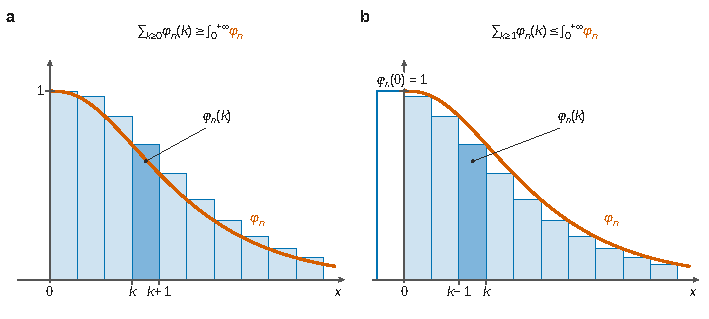
\includegraphics{figures/q23-comparaison-serie-integrale.pdf}
\caption*{Figure 2 --- Comparaison série-intégrale pour φ\_n décroissante :
rectangles de hauteur φ\_n(k) posés à droite de k (a), au-dessus de la
courbe, puis à gauche de k (b), en dessous, le terme φ\_n(0) = 1 restant
dehors}
\end{figure}

\textbf{Q24.} \emph{Changement de variable.} La fonction \(\psi:x\mapsto1-q^x\) est de classe \(\mathcal C^1\) sur \([0,+\infty[\), avec
\equationajustee{\psi'(x)=-\ln(q)\,q^x=-\ln(q)\big(1-\psi(x)\big)>0 .}
Elle est donc strictement croissante. Comme \(\psi(0)=0\) et \(\psi(x)\to1\) en \(+\infty\), elle réalise une bijection de \([0,+\infty[\) sur \([0,1[\).

La fonction \(g:u\mapsto\frac{1-u^n}{1-u}\) est continue sur \([0,1[\). Pour \(x\ge0\), en posant \(u=\psi(x)\) :
\equationajustee{\begin{aligned}
g(\psi(x))\,\psi'(x)&=\frac{1-\psi(x)^n}{1-\psi(x)}\cdot\big(-\ln(q)\big)\big(1-\psi(x)\big)\\
&=-\ln(q)\,\varphi_n(x).
\end{aligned}}
Par le théorème de changement de variable dans les intégrales généralisées, \(\int_0^1g\) et \(\int_0^{+\infty}g(\psi(x))\psi'(x)\,\mathrm dx\) sont de même nature, et égales en cas de convergence. La seconde converge, car \(\varphi_n\) est intégrable (Q22). Donc \(\int_0^1\frac{1-u^n}{1-u}\,\mathrm du\) converge et
\equationajustee{\boxed{\int_0^1\frac{1-u^n}{1-u}\,\mathrm du=-\ln(q)\int_0^{+\infty}\varphi_n(x)\,\mathrm dx.}}

\emph{Valeur.} Pour \(u\in[0,1[\), \(\frac{1-u^n}{1-u}=\sum_{j=0}^{n-1}u^j\), donc
\equationajustee{\begin{aligned}
\int_0^1\frac{1-u^n}{1-u}\,\mathrm du&=\sum_{j=0}^{n-1}\frac1{j+1}\\
&=\sum_{k=1}^n\frac1k .
\end{aligned}}
Ainsi
\equationajustee{\int_0^{+\infty}\varphi_n=\frac{1}{-\ln q}\sum_{k=1}^n\frac1k .}

\textbf{Q25.} Posons \(H_n=\sum_{k=1}^n\frac1k\) et \(I_n=\int_0^{+\infty}\varphi_n\). Par la Q24, \(I_n=\frac{H_n}{-\ln q}\). Comme \(H_n\sim\ln n\) (résultat admis), on a
\equationajustee{I_n\underset{n\to+\infty}{\sim}\frac{\ln n}{-\ln q}.}
En particulier \(I_n>0\) et \(I_n\to+\infty\). En divisant l'encadrement de la Q23 par \(I_n\) :
\equationajustee{1\le\frac{E(V_n)}{I_n}\le1+\frac1{I_n}\xrightarrow[n\to+\infty]{}1 .}
Par encadrement, \(E(V_n)\sim I_n\), et
\equationajustee{\boxed{E(V_n)\underset{n\to+\infty}{\sim}\frac{\ln n}{\ln(1/q)}.}}

\begin{center}\rule{0.5\linewidth}{0.5pt}\end{center}

Exercice 3 --- Résolution d'une équation différentielle non ordinaire

\hypertarget{partie-i---guxe9nuxe9ralituxe9s}{%
\section{Partie I - Généralités}\label{partie-i---guxe9nuxe9ralituxe9s}}

\textbf{Q26.} Par définition, \(S_\lambda\subset\mathcal D(\mathbb R,\mathbb R)\), et la fonction nulle appartient à \(S_\lambda\). Soient \(f,g\in S_\lambda\) et \(\alpha,\beta\in\mathbb R\). La fonction \(h=\alpha f+\beta g\) est dérivable et, pour tout \(x\),
\equationajustee{\begin{aligned}
h'(x)&=\alpha f(\lambda x)+\beta g(\lambda x)\\
&=h(\lambda x).
\end{aligned}}
\textbf{\(S_\lambda\) est un sous-espace vectoriel de \(\mathcal D(\mathbb R,\mathbb R)\).}

\textbf{Q27.} \((E_1)\) s'écrit \(f'=f\) : c'est une équation différentielle linéaire homogène d'ordre 1 à coefficient constant. Par le cours, ses solutions sur \(\mathbb R\) sont les \(x\mapsto Ce^x\), avec \(C\in\mathbb R\) quelconque.
\equationajustee{\boxed{S_1=\{x\mapsto Ce^x\,;\,C\in\mathbb R\}=\mathrm{Vect}(\exp).}}

\textbf{Q28.} \emph{Analyse.} Si \(f\) vérifie \((E_0)\), alors \(f'(x)=f(0)\) pour tout \(x\) ; notons \(c=f(0)\).

La fonction \(x\mapsto f(x)-cx\) a une dérivée nulle sur l'intervalle \(\mathbb R\), donc elle est constante. Il existe donc \(b\) tel que \(f(x)=cx+b\) pour tout \(x\) : \(f\) est affine.

De plus \(b=f(0)=c\), donc \(f(x)=c(x+1)\).

\emph{Synthèse.} Pour \(c\in\mathbb R\), la fonction \(x\mapsto c(x+1)\) est dérivable, de dérivée \(c\), et sa valeur en \(0\) vaut \(c\) : elle vérifie \((E_0)\).
\equationajustee{\boxed{S_0=\mathrm{Vect}(x\mapsto x+1).}}

\textbf{Q29.} \emph{Analyse.} Si \(f\) vérifie \((E_{-1})\), alors \(f'=g\) avec \(g:x\mapsto f(-x)\), qui est dérivable. Donc \(f\) est deux fois dérivable.

En appliquant \((E_{-1})\) au point \(-x\) :
\equationajustee{\begin{aligned}
f''(x)&=-f'(-x)\\
&=-f(x).
\end{aligned}}
Ainsi \(f''+f=0\), d'où \(f=\alpha\cos+\beta\sin\) avec \(\alpha,\beta\) réels. On a alors
\equationajustee{\begin{aligned}
f'(x)&=-\alpha\sin x+\beta\cos x,\\
f(-x)&=\alpha\cos x-\beta\sin x.
\end{aligned}}
Donc \(f'(x)=f(-x)\) pour tout \(x\) équivaut à \((\beta-\alpha)(\cos x+\sin x)=0\) pour tout \(x\). En \(x=0\), cela impose \(\beta=\alpha\).

\emph{Synthèse.} Pour \(f=\alpha(\cos+\sin)\), on a \(f'(x)=\alpha(\cos x-\sin x)=f(-x)\).
\equationajustee{\boxed{S_{-1}=\mathrm{Vect}(\cos+\sin).}}

\hypertarget{partie-ii---solutions-duxe9veloppables-en-suxe9rie-entiuxe8re}{%
\section{Partie II - Solutions développables en série entière}\label{partie-ii---solutions-duxe9veloppables-en-suxe9rie-entiuxe8re}}

Dans cette partie, \(\lambda\ne0\).

\textbf{Q30.} Posons \(c_n=\frac{\lambda^{n(n-1)/2}}{n!}\), non nul car \(\lambda\ne0\). Avec les valeurs absolues, et puisque \(|\lambda|\le1\) :
\equationajustee{\begin{aligned}
\left|\frac{c_{n+1}}{c_n}\right|&=\frac{|\lambda|^{n}}{n+1}\\
&\le\frac1{n+1}.
\end{aligned}}
Ce quotient tend vers \(0\). Par la règle de d'Alembert, \(\boxed{R=+\infty}\). (On peut aussi majorer \(|c_nx^n|\le|x|^n/n!\).)

\textbf{Q31.} La série entière définissant \(\varphi\) a un rayon infini (Q30). Par le théorème de dérivation terme à terme d'une série entière sur son intervalle ouvert de convergence, \(\varphi\) est dérivable sur \(\mathbb R\) et, pour tout \(x\),
\equationajustee{\begin{aligned}
\varphi'(x)&=\sum_{n\ge1}\lambda^{\frac{n(n-1)}2}\frac{x^{n-1}}{(n-1)!}\\
&=\sum_{m\ge0}\lambda^{\frac{m(m+1)}2}\frac{x^m}{m!}.
\end{aligned}}
Le rayon étant infini, la série en \(\lambda x\) converge aussi :
\equationajustee{\varphi(\lambda x)=\sum_{m\ge0}\lambda^{\frac{m(m-1)}2+m}\frac{x^m}{m!}.}
Comme \(\frac{m(m-1)}2+m=\frac{m(m+1)}2\), on a \(\varphi'(x)=\varphi(\lambda x)\) pour tout \(x\) : \(\boxed{\varphi\in S_\lambda}\).

\textbf{Q32.} La série \(\sum a_nx^n\) a un rayon infini. Par dérivation terme à terme, \(f\) est dérivable sur \(\mathbb R\) et
\equationajustee{f'(x)=\sum_{n\ge0}(n+1)a_{n+1}x^n .}
Par ailleurs, la série \(\sum a_n(\lambda x)^n\) converge pour tout \(x\), donc
\equationajustee{f(\lambda x)=\sum_{n\ge0}\lambda^na_nx^n .}
Ces deux séries entières sont de rayon infini. Si \(f'(x)=f(\lambda x)\) pour tout \(x\), l'unicité du développement en série entière donne
\equationajustee{\boxed{\forall n\in\mathbb N,\quad(n+1)a_{n+1}=\lambda^na_n.}}

\textbf{Q33.} \emph{Sens direct.} Supposons \(f\) solution. Montrons par récurrence sur \(n\), à l'aide de la Q32, que
\equationajustee{a_n=a_0\frac{\lambda^{n(n-1)/2}}{n!}.}
C'est vrai pour \(n=0\). Si c'est vrai au rang \(n\), alors
\equationajustee{\begin{aligned}
a_{n+1}&=\frac{\lambda^n}{n+1}a_n\\
&=a_0\frac{\lambda^{n(n+1)/2}}{(n+1)!}.
\end{aligned}}
Donc \(f=a_0\varphi\in\mathrm{Vect}(\varphi)\), où \(a_0=f(0)\) est un réel quelconque.

\emph{Réciproque.} \(\varphi\in S_\lambda\) (Q31) et \(S_\lambda\) est un sous-espace vectoriel (Q26), donc \(\mathrm{Vect}(\varphi)\subset S_\lambda\).
\equationajustee{\boxed{f\text{ est solution de }(E_\lambda)\iff f\in\mathrm{Vect}(\varphi).}}

\hypertarget{partie-iii---duxe9termination-de-toutes-les-solutions}{%
\section{Partie III - Détermination de toutes les solutions}\label{partie-iii---duxe9termination-de-toutes-les-solutions}}

Ici \(\lambda\ne0\), \(|\lambda|\le1\) et \(f\in S_\lambda\).

\textbf{Q34.} Notons \(\mathcal P(n)\) : « \(f\) est de classe \(\mathcal C^n\) sur \(\mathbb R\) et \(f^{(n)}(t)=\lambda^{n(n-1)/2}f(\lambda^nt)\) pour tout \(t\) ».

\begin{itemize}
\tightlist
\item
  Initialisation, \(n=0\) : \(f\) est dérivable, donc continue, et \(f^{(0)}(t)=f(t)=\lambda^0f(\lambda^0t)\).
\item
  Hérédité : supposons \(\mathcal P(n)\). La fonction \(f\) est dérivable, donc \(t\mapsto f(\lambda^nt)\) l'est, de dérivée \(t\mapsto\lambda^nf'(\lambda^nt)\).
  Par \((E_\lambda)\) au point \(\lambda^nt\), on a \(f'(\lambda^nt)=f(\lambda^{n+1}t)\). Donc \(f^{(n)}\) est dérivable et
\end{itemize}

\equationajustee{\begin{aligned}
f^{(n+1)}(t)&=\lambda^{\frac{n(n-1)}2+n}f(\lambda^{n+1}t)\\
&=\lambda^{\frac{(n+1)n}2}f(\lambda^{n+1}t).
\end{aligned}}
Cette fonction est continue, car \(f\) l'est. Ainsi \(f^{(n)}\) est de classe \(\mathcal C^1\), donc \(f\) est de classe \(\mathcal C^{n+1}\) : \(\mathcal P(n+1)\) est vraie.
\equationajustee{\boxed{\forall n\in\mathbb N,\ f\in\mathcal C^n(\mathbb R)\text{ et }f^{(n)}(t)=\lambda^{\frac{n(n-1)}2}f(\lambda^nt).}}
En particulier, \(f\) est de classe \(\mathcal C^\infty\).

\textbf{Q35.} \(f\) est continue sur le segment \([-a,a]\), donc bornée : posons \(M_a=\sup_{[-a,a]}|f|\).

Soit \(t\in[-a,a]\). Comme \(|\lambda|\le1\), on a \(|\lambda^{n+1}t|\le|t|\le a\) et \(|\lambda|^{n(n+1)/2}\le1\). Par la Q34, \(|f^{(n+1)}(t)|\le M_a\).

Comme \(|x-t|\le2a\), on obtient, pour tout \(n\) :
\equationajustee{\sup_{t\in[-a,a]}|g_n(t)|\le\frac{(2a)^n}{n!}M_a .}
Le majorant ne dépend pas de \(t\) et tend vers \(0\) quand \(n\to+\infty\) (croissances comparées).

\textbf{\((g_n)\) converge uniformément vers \(0\) sur \([-a,a]\).}

\textbf{Q36.} \(f\) est de classe \(\mathcal C^\infty\) (Q34). Fixons \(x\in\mathbb R\) et prenons \(a=|x|+1\), de sorte que \(x\in[-a,a]\).

Tout \(t\) entre \(0\) et \(x\) est dans \([-a,a]\). Par la formule de Taylor admise, puis par la Q35 :
\equationajustee{\begin{aligned}
\left|f(x)-\sum_{k=0}^n\frac{f^{(k)}(0)}{k!}x^k\right|&=\left|\int_0^xg_n(t)\,\mathrm dt\right|\\
&\le|x|\sup_{[-a,a]}|g_n|.
\end{aligned}}
Le majorant tend vers \(0\) quand \(n\to+\infty\). Ainsi, pour tout réel \(x\),
\equationajustee{f(x)=\sum_{k=0}^{+\infty}\frac{f^{(k)}(0)}{k!}x^k .}
La série entière converge sur \(\mathbb R\), donc son rayon est infini.
\equationajustee{\boxed{f\text{ est \text{développable} en \text{série} \text{entière} sur }\mathbb R.}}
(Par la Q34 en \(t=0\), \(f^{(k)}(0)=\lambda^{k(k-1)/2}f(0)\), donc \(f=f(0)\varphi\).)

\textbf{Q37.} \emph{Cas \(\lambda\ne0\).} Toute \(f\in S_\lambda\) est la somme d'une série entière de rayon infini (Q36), donc \(f\in\mathrm{Vect}(\varphi)\) (Q33). Réciproquement, \(\mathrm{Vect}(\varphi)\subset S_\lambda\).

Ainsi \(S_\lambda=\mathrm{Vect}(\varphi)\), avec \(\varphi(0)=1\), donc \(\varphi\ne0\) et la famille \((\varphi)\) est libre.

\emph{Cas \(\lambda=0\).} \(S_0=\mathrm{Vect}(x\mapsto x+1)\) (Q28).
\equationajustee{\boxed{\forall\lambda\in[-1,1],\quad\dim S_\lambda=1.}}

\textbf{FIN}

\end{document}
